% Universidade Federal de Campina Grande
% Modelo de Proposta de Disserta��o de Mestrado em Ciencia da Computacao
%
% Feito por: Ana Cristina Alves de Oliveira
% (cristina@dsc.ufcg.edu.br - orientador: Francisco Brasileiro)
% Fevereiro de 2006

% E necessario o arquivo "algorithm.sty", se for construir algoritmos

% Adaptado por: Leandro Dias da Silva
% (leandrodias@ic.ufal.br - Coordenador do PPGI)
% Junho de 2013

% readaptado por: Ailton Felix, Lucas Lins, Marcelo Oliveira
% (oliveiramc@ic.ufal.br - Coordenador do PPGI)
% em Julho de 2018

\documentclass[a4paper,titlepage,12pt]{article}

\usepackage{color}
\usepackage{longtable}

%\usepackage[portuges,english]{babel}

%Portuguese-specific commands
%--------------------------------------
\usepackage[english,brazil,portuguese]{babel}
%--------------------------------------
 
%Acentuação em UTF8
\usepackage[utf8]{inputenc}            % 
%\usepackage[latin1]{inputenc}

\usepackage{times}
%\usepackage[latin1]{inputenc}
\usepackage[T1]{fontenc}
\usepackage{fancyheadings}
\usepackage{fancyvrb}

\usepackage{algorithmic}
\usepackage[nothing]{algorithm}
\usepackage{latexsym}
\usepackage{indentfirst}                 % indenta os primeiros parágrafos
\usepackage{amsmath}  %texto no modo math
\usepackage[colorlinks,pdftex,pdfpagelabels=false]{hyperref} % Inclusão de links  

\usepackage{graphicx,url}

\sloppy

% Comandos de estilo e espacamento ----------------------------------------
\newlength{\defbaselineskip}
\setlength{\defbaselineskip}{\baselineskip}
\newcommand{\setlinespacing}[1]%
           {\setlength{\baselineskip}{#1 \defbaselineskip}}

\setcounter{topnumber}{2}
\renewcommand{\topfraction}{.7}
\setcounter{bottomnumber}{1}
\renewcommand{\bottomfraction}{.3}
\setcounter{totalnumber}{3}
\renewcommand{\textfraction}{.2}
\renewcommand{\floatpagefraction}{.5}
\setcounter{dbltopnumber}{2}
\renewcommand{\dbltopfraction}{.7}
\renewcommand{\dblfloatpagefraction}{.5}
%
\oddsidemargin -28pt
\evensidemargin -28pt
\marginparwidth 50pt
\marginparsep 5pt
\topmargin -27pt
\hoffset 15mm
\textheight 237mm
\textwidth 155mm
\renewcommand{\baselinestretch}{1.5}
%

% ------------------------------------------------------------------------

%%%%%  Ambiente de redefinicoes para contrucao de Algoritmos
% Apenas usar se precisar fazer algoritmos

\renewcommand{\algorithmicend}{\textbf{fim}}
\renewcommand{\algorithmicwhen}{\textbf{quando}}
\renewcommand{\algorithmicprimitive}{\textbf{in�cio}}
\renewcommand{\algorithmicendprimitive}{\textbf{fim}}
\renewcommand{\algorithmicendwhen}{\textbf{fim}}
\renewcommand{\algorithmicif}{\textbf{se}}
\renewcommand{\algorithmicthen}{\textbf{ent\~{a}o}}
\renewcommand{\algorithmicelse}{\textbf{sen\~{a}o}}
\renewcommand{\algorithmicendif}{\textbf{fim-se}}
\renewcommand{\algorithmicelsif}{\algorithmicelse\ \algorithmicif}
\renewcommand{\algorithmicendif}{\algorithmicend\ \algorithmicif}
\renewcommand{\algorithmicfor}{\textbf{para}}
\renewcommand{\algorithmicforall}{\textbf{paratodos}}
\renewcommand{\algorithmicdo}{\textbf{fa\c{c}a}}
\renewcommand{\algorithmicendfor}{\algorithmicend\ \algorithmicfor}
\renewcommand{\algorithmicwhile}{\textbf{enquanto}}
\renewcommand{\algorithmicendwhile}{\algorithmicend\ \algorithmicwhile}
\renewcommand{\algorithmicloop}{\textbf{loop}}
\renewcommand{\algorithmicendloop}{\algorithmicend\ \algorithmicloop}
\renewcommand{\algorithmicrepeat}{\textbf{repita}}
\renewcommand{\algorithmicuntil}{\textbf{at\'{e}}}
\renewcommand{\algorithmicwaituntil}{\textbf{espera at�}}
\floatname{algorithm}{Algoritmo}

%%%%%%

% Color definitions (RGB model)
\definecolor{mycolor1}{rgb}{0.753,0.753,0.753}

\begin{document}

% Primeira Folha do Documento %%%%%%%%%%%%%%%%%%%%%%%%%%%%%%%%%%%%%%%%%%%%%

\pagestyle{empty}

\begin{center}
{\textbf{\Large \textsc{Universidade Federal de Alagoas}}}
\end{center}

\begin{center}
\textbf{{\Large \textsc{Instituto de Computação}}}
\end{center}

\begin{center}
{\large \textsc{\textbf{Coordenação de Pós-Graduação em Informática}}}
\end{center}

~\\ \\

\begin{center}
{\LARGE \textsc{\textbf{Proposta de Dissertação de
Mestrado}}}
\end{center}

~\\ \\

\begin{center}
{\Large \textsc{\textbf{<<Título da Proposta>>}}}
\end{center}

~\\ \\

\begin{center}
\textbf{\textsc{Mestrando(a)} \\
\textsc{<<Seu Nome>>}}
\end{center}

\begin{center}
\textbf{\textsc{Orientador(a)} \\
\textsc{<<Nome(s) do(s) Orientador(es)>>}}
\end{center}

~\\ \\ \\

\begin{center}
\textbf{{\large \textsc{Maceió, AL}}
\\
{\large \textsc{<<Mes>> - <<Ano>>}}}
\end{center}

\newpage
\cleardoublepage

%%%%%%%%%%%%%%%%%%%%%%%%%%%%%%%%%%%%%%%%%%%%%%%%%%%%%%%%%%%%%%%%%%%%%%%%%%%%%%%%

\selectlanguage{portuguese}

% ConFigura os n�meros das p�ginas para algarismos romanos
\pagestyle{plain}
\pagenumbering{roman}

\listoffigures
\newpage

\listoftables
\newpage
% Inclui a lista de algoritmos
\incluilistadealgoritmos

\tableofcontents
\newpage

% Corpo do documento -------------------

% ConFigura os n�meros das p�ginas para algarismos indo-arabicos
\pagestyle{plain}
\setcounter{page}{1}
\pagenumbering{arabic}

%%%%%%%%%%%%%%%%%%%%%%%%%%%%%%%%%%%%%%%%%%%%%%%%%%%%%%%%%%%%%%%%%%%%%%%%%%%%%%%%
%% Definicao do cabecalho: secao do lado esquerdo e numero da pagina do lado direito
\pagestyle{fancy}
\addtolength{\headwidth}{\marginparsep}\addtolength{\headwidth}{\marginparwidth}\headwidth
= \textwidth
%\renewcommand{\sectionmark}[1]{\markboth{#1}{}}
\renewcommand{\sectionmark}[1]{\markright{\thesection\ #1}}\lhead[\fancyplain{}{\bfseries\thepage}]%
         {\fancyplain{}{\emph{\rightmark}}}\rhead[\fancyplain{}{\bfseries\leftmark}]%
             {\fancyplain{}{\bfseries\thepage}}\cfoot{}

%%%%%%%%%%%%%%%%%%%%%%%%%%%%%%%%%%%%%%%%%%%%%%%%%%%%%%%%%%%%%%%%%%%%%%%%%%%%%%%%


\section{Introdução}
\label{sec:introdu}

Na introdução você deve contextualizar o problema que estará estudando. Em particular, você deve descrever brevemente a área na qual estará trabalhando e introduzir de forma clara os problemas da área relevantes ao seu trabalho. Observe que a seção não fala de soluções mas de problemas existindo na área de interesse.
Sem contar apêndices e referências bibliográficas, uma proposta de dissertação de mestrado geralmente contêm uma dezena de páginas.

\section{Objetivo Geral e Específico}
\label{sec:objetivo}

Nesta seção, você deve falar da solução que você propõe aos problemas apresentados anteriormente. O enfoque é sobre ``o quê‘‘ você vai fazer.

\section{Relevância da Proposta}
\label{sec:relev}

Aqui, o enfoque é o "porquê". Você pode se concentrar em responder à seguinte pergunta: "Se meu trabalho for bem sucedido, o que terá mudado na área sob estudo?". Em outras palavras, quais são as contribuições planejadas?

\section{Desenvolvimento (ou Materiais e Métodos)}
\label{sec:metodologia}


Aqui o enfoque é o "como".  Quais são os passos que deverão ser desenvolvidos, e em que ordem, para que o trabalho seja feito. Uma tabela semelhante à Tabela~\ref{tab:atividades} pode ser utilizada para apoiar a apresentação.

\begin{table}[H]
\caption{Atividades planejadas.}
\label{tab:atividades}
 \small
  \begin{center}
    \begin{tabular}{|c||p{13cm}|} \hline
      {\bf Atividade}   &{\bf Descrição} \\\hline
      {\bf 1}   & Realizar uma pesquisa bibliográfica sobre as soluções existentes para o problema de \textit{xpto}.  \\\hline
      {\bf 2}   & Elaborar relatório técnico contendo a avaliação das soluções encontradas. \\\hline
      {\bf 3}   & Levantar os requisitos básicos da solução desejada. \\\hline
      {\bf 3.1}   & Definir um esboço de uma solução a ser implementada que atenda aos requisitos levantados. \\\hline
      {\bf 4}   & Elaborar o projeto da solução e definir a linguagem de programação a ser usada para implementar a ferramenta. O processo de desenvolvimento utilizado será baseado no Processo Unificado, utilizando UML como linguagem de modelagem. \\\hline
      {\bf 4.1}   & Fazer o levantamento detalhado de requisitos funcionais da ferramenta, gerando um modelo de Análise. \\\hline
      {\bf 4.2}   & Definir a arquitetura da ferramenta, gerando um modelo arquitetural. \\\hline
      {\bf 4.3}   & Definir a linguagem de programação na qual a ferramenta será implementada. \\\hline
      {\bf 4.4}   & Elaborar o projeto da ferramenta, gerando um modelo de projeto. \\\hline
      {\bf 5}  & Implementar a ferramenta utilizando a linguagem de programação escolhida. Serão utilizados testes de unidade durante esta fase. \\\hline
      {\bf 6}  & Elaborar um artigo contendo a avaliação da ferramenta. \\\hline
      {\bf 7}  & Elaborar a redação da dissertação de mestrado. \\\hline
      {\bf 8}  & Defender a dissertação de mestrado. \\\hline
    \end{tabular}
  \end{center}
%  \normalsize
\end{table}

\newpage


\section{Cronograma de Execução}
\label{sec:cronograma}

O cronograma apresenta a dimensão "quando". As atividades mencionadas na Metodologia devem ser cronogramadas, incluindo data de início, data final, dependências entre atividades.
Um exemplo de cronograma é apresentado na Tabela~\ref{tab:cronograma}.

\begin{table}[ht]
\caption{Cronograma do projeto de pesquisa.} \label{tab:cronograma}
%  \scriptsize
  \begin{center}
    \begin{tabular}{|c|c||c|c|c|c|c|c|c|c|c|c|c|c|c|c|} \hline
                       & & \multicolumn{14}{c|}{ {\bf Atividade } } \\\hline \hline
      {\bf Ano}  &{\bf M�s}  &{\bf 1}  &{\bf 2}  &{\bf 3} &{\bf 4}  &{\bf 5}  &{\bf 6}  &{\bf 7} &{\bf 8}  &{\bf 9}  &{\bf 10} &{\bf 11}  &{\bf 12}  &{\bf 13}  &{\bf 14}\\\hline
      {\bf 2005} &{\bf Jun}  & X       & X       &        &         &         &         &        &         &         &         &          &          &          &        \\\hline
      {\bf 2005} &{\bf Jul}  & X       &         & X      &         &         &         &        &         &         &         &          &          &          &        \\\hline
      {\bf 2005} &{\bf Ago}  & X       &         &        & X       &         &         &        &         &         &         &          &          &          &        \\\hline
      {\bf 2005} &{\bf Set}  & X       &         &        &         & X       &         &        &         &         &         &          &          &          &        \\\hline
      {\bf 2005} &{\bf Out}  & X       &         &        &         & X       &         &        &         &         &         &          &          &          &        \\\hline
      {\bf 2005} &{\bf Nov}  & X       &         &        &         & X       &         &        &         &         &         &          &          &          &        \\\hline
      {\bf 2005} &{\bf Dez}  & X       &         &        &         &         & X       &        &         &         &         &          &          &          &        \\\hline
      {\bf 2006} &{\bf Jan}  & X       &         &        &         &         &         & X      &         &         &         &          &          &          &        \\\hline
      {\bf 2006} &{\bf Fev}  & X       &         &        &         &         &         & X      &         &         &         &          &          &          &        \\\hline
      {\bf 2006} &{\bf Mar}  &         &         &        &         &         &         &        & X       & X       &         &          &          &          &        \\\hline
      {\bf 2006} &{\bf Abr}  &         &         &        &         &         &         &        &         &         & X       &          &          &          &        \\\hline
      {\bf 2006} &{\bf Mai}  &         &         &        &         &         &         &        &         &         & X       &          &          &          &        \\\hline
      {\bf 2006} &{\bf Jun}  &         &         &        &         &         &         &        &         &         &         & X        &          &          &        \\\hline
      {\bf 2006} &{\bf Jul}  &         &         &        &         &         &         &        &         &         &         &          & X        &          &        \\\hline
      {\bf 2006} &{\bf Ago}  &         &         &        &         &         &         &        &         &         &         &          &          &  X       &        \\\hline
      {\bf 2006} &{\bf Set}  &         &         &        &         &         &         &        &         &         &         &          &          &  X       &        \\\hline
      {\bf 2006} &{\bf Out}  &         &         &        &         &         &         &        &         &         &         &          &          &  X       &        \\\hline
      {\bf 2006} &{\bf Nov}  &         &         &        &         &         &         &        &         &         &         &          &          &  X       &        \\\hline
      {\bf 2006} &{\bf Dez}  &         &         &        &         &         &         &        &         &         &         &          &          &          & X      \\\hline
    \end{tabular}
  \end{center}
%  \normalsize
\end{table}

\section{Resultados Preliminares (Opcional)}

\newpage

%%%%%%%%%%%%%%%%%%%%%%%%%%%%%%%%%%%%%%%%%%%%%%%%%%%%%%%%%%%%%%%%%%%%%%%%%%%%%%%%
%% BIbliografia

\bibliographystyle{alpha} % estilo de bibliografia
\bibliography{referencias} % arquivos com as entradas bib.

%%%%%%%%%%%%%%%%%%%%%%%%%%%%%%%%%%%%%%%%%%%%%%%%%%%%%%%%%%%%%%%%%%%%%%%%%%%%%%%%

\newpage


\appendix
\section{Título do apêndice A}
\label{ape:apeA}

Incluir o texto do apêndice aqui. Embora não sejam obrigatórios, os apêndices geralmente incluem um levantamento do estado da arte, descrição de soluções existentes, etc.

Exemplo de inserção de algoritmos: Algoritmo~\ref{alg:escalonamento}. Este utiliza uma heur\'{\i}stica
simples, como mostra o Algoritmo~\ref{alg:heuristica}.

% Algoritmo de escalonamento -------

\begin{algorithm}
\caption{Escalonamento usando sistema de reputação}
\label{alg:escalonamento}
\small
\begin{algorithmic}

\IF {máquina M for local} \STATE $Cr_{P}(M) = 1$ \ELSE \STATE
$Cr_{P}(M) = 0$ \ENDIF

\STATE Ordene máquinas na fila pela credibilidade

\STATE /* Fase 1 */ \WHILE {(houver máquinas ociosas) $\land$
(houver tarefas não escalonadas)}
    \STATE escalone
\ENDWHILE

\STATE /* Fase 2 */ \WHILE {(houver tarefa que não atingiu a
$Cr_{alvo}$) $\land$ (existir máquina ociosa)}

    \IF {houver tarefa não escalonada na fila}
        \STATE escalone
    \ELSE
        \STATE escalone seguindo \textbf{heurística}
    \ENDIF

\ENDWHILE

\end {algorithmic}
\end {algorithm}

% Final do Algoritmo


% Heuristica de escalonamento -------

\begin{algorithm}
\caption{Heurística simples de escalonamento} \label{alg:heuristica}
\small
\begin{algorithmic}

\IF {(houver tarefa T cuja $Cr_{W}(T) \leq Cr_{alvo}$)}
    \STATE escolha a tarefa cuja credibilidade é mais próxima de $Cr_{alvo}$
\ENDIF

\end {algorithmic}
\end {algorithm}


Exemplo de inserção de figura e de referência: a Figura \ref{fig:ourgrid} representa a comunidade OurGrid \cite{Paranhos:03}.

\begin{figure}[ht]
\centering
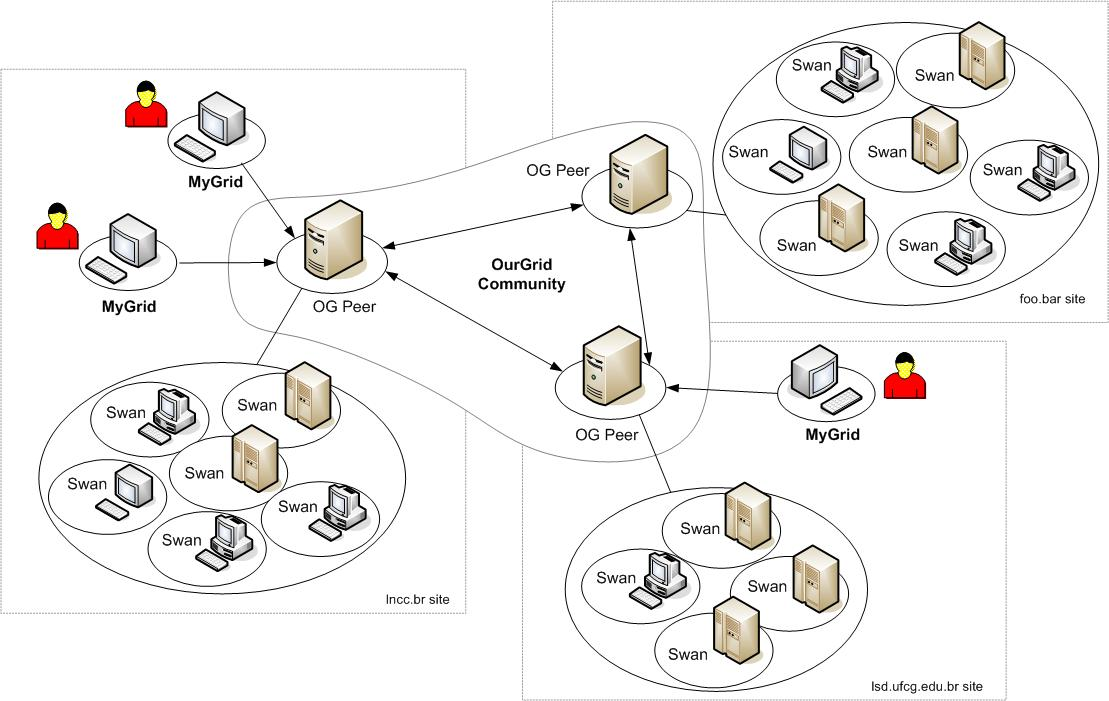
\includegraphics[width=.80\textwidth]{figs/ourgrid.jpg}
\caption{Comunidade OurGrid.} \label{fig:ourgrid}
\end{figure}

% Final do Algoritmo


\section{Título do apêndice B}
\label{ape:apeB}

Incluir o texto do apêndice aqui, caso haja.


\end{document}
